% !TeX program = pdflatex
\documentclass[aspectratio=169,t]{beamer}

% Idioma e Codificacao
\usepackage[brazilian]{babel}
\usepackage{booktabs}
\usepackage{array}
\usepackage{listings}
\usepackage{amsmath}
\usepackage{amssymb}
\usepackage{graphicx}
\usepackage{tikz}
\usetikzlibrary{shapes,arrows,positioning,calc,shapes.multipart}

% Carrega o Tema Modelo dos Scouts (Widescreen 16:9, Nunito Sans)
\usetheme{scouts}

% Redefine as Margens para Maximizar a Area Util de Escrita (140mm de largura util em 16:9)
\setbeamersize{text margin left=10mm, text margin right=10mm}

% Ajuste de Altura e Posicao do Titulo do Slide: Reduz Espacamento com o Topo (Cabecalho)
\setbeamerfont{frametitle}{series=\bfseries,size=\large}
\setbeamertemplate{frametitle}{%
  \vspace*{-2.5mm}% Reduz o espacamento entre o cabecalho da secao e o titulo do frame
  \begin{beamercolorbox}[wd=\textwidth,sep=0mm,left]{title}%
    \parbox[t]{\textwidth}{%
      \usebeamerfont{frametitle}\insertframetitle\strut%
    }%
  \end{beamercolorbox}%
  \vspace*{1.5mm}%
}

% Ajuste da Fonte do Comando \alert para Manter Hierarquia Visual Subordinada ao Titulo
\setbeamerfont{alerted text}{series=\bfseries,size=\footnotesize}

% Ajuste do Rodape para Liberar Mais Espaco Vertical
\setbeamertemplate{footline}{%
  \begin{beamercolorbox}[wd=\paperwidth,dp=1mm,ht=2.5mm,leftskip=10mm,rightskip=10mm]{footline}%
    \usebeamerfont{title in head/foot}\hfill%
  \end{beamercolorbox}%
}

% Ajuste Global de Fontes Beamer para Evitar Estouro de Listas Aninhadas
\setbeamerfont{itemize/enumerate body}{size=\scriptsize}
\setbeamerfont{itemize/enumerate subbody}{size=\scriptsize}
\setbeamerfont{itemize/enumerate subsubbody}{size=\tiny}
\setbeamerfont{item}{size=\scriptsize}
\setbeamerfont{subitem}{size=\tiny}

% Definicao de linguagem JavaScript/JSON/MongoSH para o listings
\lstdefinelanguage{mongosh}{
  keywords={use, show, db, dbs, collections, aggregate, match, group, project, sort, limit, skip, unwind, lookup, facet, bucket, count, sum, avg, min, max, push, addToSet, first, last, round, concat, toString, cond, year, month, dayOfMonth, size, ObjectId, ISODate, true, false, null},
  sensitive=true,
  comment=[l]{//},
  morecomment=[s]{/*}{*/},
  morestring=[b]",
  morestring=[b]'
}

% Configuracao para Codigo-Fonte (MongoSH / Python / JSON)
\lstset{
    basicstyle=\fontsize{5.2pt}{6.3pt}\selectfont\ttfamily,
    keywordstyle=\bfseries\color{ScoutNavy},
    stringstyle=\color{ScoutGreen},
    commentstyle=\itshape\color{gray},
    backgroundcolor=\color{black!3},
    frame=single,
    rulecolor=\color{black!15},
    breaklines=true,
    breakatwhitespace=true,
    showstringspaces=false,
    tabsize=2,
    aboveskip=2pt,
    belowskip=1pt,
    literate={á}{{\'a}}1 {ã}{{\~a}}1 {â}{{\^a}}1 {à}{{\`a}}1
             {é}{{\'e}}1 {ê}{{\^e}}1 {í}{{\'i}}1 {ó}{{\'o}}1
             {õ}{{\~o}}1 {ô}{{\^o}}1 {ú}{{\'u}}1 {ç}{{\c{c}}}1
             {Á}{{\'A}}1 {Ã}{{\~A}}1 {É}{{\'E}}1 {Í}{{\'I}}1
             {Ó}{{\'O}}1 {Õ}{{\~O}}1 {Ú}{{\'U}}1 {Ç}{{\c{C}}}1
}

% Metadados Institucionais
\author{Prof. Me. Reginaldo Fernandes}
\institute{Instituto Federal do Ceará -- Campus Tauá \\ Tecnologia em Análise e Desenvolvimento de Sistemas}
\title{Bancos de Dados Não-Relacionais}
\subtitle{Aula 08: MongoDB Aggregation Framework -- Pipelines Analíticos e Business Intelligence}
\date{10 de Novembro de 2026}

\begin{document}
\shorthandoff{"}

% ------------------------------------------------------------------------------
% Capa da Apresentacao
% ------------------------------------------------------------------------------
\changecolours[inverse]{ScoutGreen}
\frame[plain]{\titlepage}

% ------------------------------------------------------------------------------
% Sumario Executivo da Aula
% ------------------------------------------------------------------------------
\changecolours{ScoutGreen}
\begin{frame}{Agenda do Encontro}
  \vspace{0.3cm}
  \tableofcontents
\end{frame}

% ------------------------------------------------------------------------------
% Modulos da Aula
% ------------------------------------------------------------------------------
% !TeX root = main.tex
\changecolours{ScoutGreen}
\shorthandoff{"}
\section[Paradigma de Processamento em Pipeline]{Paradigma de Processamento em Pipeline (Dataflow)}

% ------------------------------------------------------------------------------
\begin{frame}[fragile]{Além do CRUD: O Gargalo da Análise de Dados no Cliente}
  \vspace{0.1cm}
  \begin{columns}[t,onlytextwidth]
    \begin{column}{0.48\textwidth}
      \alert{Limitações do Método \texttt{find()} Convencional}\par
      \footnotesize
      \begin{itemize}
        \item O comando \lstinline[language=mongosh, basicstyle=\footnotesize\ttfamily]|find()| realiza buscas pontuais e filtros simples.
        \item \textbf{Incapacidade Analítica:} Não calcula métricas agregadas (somas, médias, desvios) nativamente no servidor.
        \item \textbf{Processamento no Cliente:} Para calcular o faturamento mensal, a aplicação precisa baixar $10.000$ pedidos inteiros.
        \item \textbf{Impacto:} Saturação da rede e esgotamento da memória RAM dos microsserviços.
      \end{itemize}
    \end{column}
    \begin{column}{0.48\textwidth}
      \alert{A Solução: Aggregation Framework}\par
      \footnotesize
      \begin{itemize}
        \item \textbf{Processamento no Servidor:} Execução nativa em C++ no motor WiredTiger, junto aos dados.
        \item \textbf{Arquitetura Dataflow:} Esteira ordenada de estágios onde cada saída é a entrada do próximo estágio.
        \item \textbf{Economia de Rede:} O servidor processa gigabytes de histórico e entrega ao cliente apenas kilobytes sintetizados.
      \end{itemize}
    \end{column}
  \end{columns}
\end{frame}

% ------------------------------------------------------------------------------
\begin{frame}{Conceito de Aggregation Pipeline: Fluxo Sequencial}
  \vspace{-0.15cm}
  \centering
  \begin{tikzpicture}[
    scale=0.78, transform shape,
    stagebox/.style={
      rectangle, draw=ScoutNavy, fill=ScoutNavy!10, rounded corners=3pt,
      line width=0.8pt, font=\scriptsize\bfseries, align=center, inner sep=3.5pt
    },
    filterbox/.style={
      rectangle, draw=ScoutGreen!85!black, fill=ScoutGreen!15, rounded corners=3pt,
      line width=0.8pt, font=\scriptsize\bfseries, align=center, inner sep=3.5pt
    },
    groupbox/.style={
      rectangle, draw=ScoutTeal!85!black, fill=ScoutTeal!20, rounded corners=3pt,
      line width=0.8pt, font=\scriptsize\bfseries, align=center, inner sep=3.5pt
    },
    sortbox/.style={
      rectangle, draw=ScoutPurple!85!black, fill=ScoutPurple!15, rounded corners=3pt,
      line width=0.8pt, font=\scriptsize\bfseries, align=center, inner sep=3.5pt
    },
    flowarrow/.style={->, >=stealth, line width=1.1pt, ScoutNavy!80},
    metaflow/.style={font=\tiny\bfseries\color{ScoutNavy!90}, align=center}
  ]
    \node[stagebox] (n0) at (0, 0) {Coleção Física\\\textbf{\texttt{pedidos}}\\\tiny 10.000 docs};
    \node[filterbox] (n1) at (3.4, 0) {Estágio 1\\\textbf{\texttt{\$match}}\\\tiny status: entregue};
    \node[groupbox] (n2) at (6.8, 0) {Estágio 2\\\textbf{\texttt{\$group}}\\\tiny agrupa por mês};
    \node[sortbox] (n3) at (10.2, 0) {Estágio 3\\\textbf{\texttt{\$sort}}\\\tiny ordem temporal};
    \node[stagebox, fill=ScoutGreen!25] (n4) at (13.5, 0) {Saída Final\\\textbf{Relatório}\\\tiny 12 registros};

    \draw[flowarrow] (n0) -- node[above=1pt, metaflow] {Stream} (n1);
    \draw[flowarrow] (n1) -- node[above=1pt, metaflow] {7.500 docs} (n2);
    \draw[flowarrow] (n2) -- node[above=1pt, metaflow] {12 meses} (n3);
    \draw[flowarrow] (n3) -- node[above=1pt, metaflow] {Final} (n4);
  \end{tikzpicture}

  \vspace{0.15cm}
  \begin{columns}[t,onlytextwidth]
    \begin{column}{0.48\textwidth}
      \alert{Princípio da Imutabilidade}\par
      \footnotesize
      \begin{itemize}
        \item Os documentos na coleção física original permanecem totalmente inalterados.
        \item Cada estágio gera documentos efêmeros intermediários na memória.
      \end{itemize}
    \end{column}
    \begin{column}{0.48\textwidth}
      \alert{Processamento em Fluxo (\textit{Streaming})}\par
      \footnotesize
      \begin{itemize}
        \item Documentos fluem continuamente de um estágio para o próximo.
        \item Descarte precoce de campos e documentos libera memória RAM de imediato.
      \end{itemize}
    \end{column}
  \end{columns}
\end{frame}

% ------------------------------------------------------------------------------
\begin{frame}[fragile]{Equivalência Conceitual: SQL Relacional vs MongoDB Pipeline}
  \vspace{0.05cm}
  \begin{columns}[t,onlytextwidth]
    \begin{column}{0.40\textwidth}
      \alert{Mapeamento de Operações}\par
      \vspace{0.4cm}
      \scriptsize
      \begin{tabular}{@{}ll@{}}
        \toprule
        \textbf{SQL Relacional} & \textbf{Pipeline MongoDB} \\
        \midrule
        \textbf{WHERE}    & \lstinline[language=mongosh, basicstyle=\footnotesize\ttfamily]|$match| \\
        \textbf{SELECT}   & \lstinline[language=mongosh, basicstyle=\footnotesize\ttfamily]|$project| \\
        \textbf{GROUP BY} & \lstinline[language=mongosh, basicstyle=\footnotesize\ttfamily]|$group| \\
        \textbf{HAVING}   & \lstinline[language=mongosh, basicstyle=\footnotesize\ttfamily]|$match| \textnormal{\textit{(pós)}} \\
        \textbf{ORDER BY} & \lstinline[language=mongosh, basicstyle=\footnotesize\ttfamily]|$sort| \\
        \textbf{LIMIT}    & \lstinline[language=mongosh, basicstyle=\footnotesize\ttfamily]|$limit| \\
        \textbf{OFFSET}   & \lstinline[language=mongosh, basicstyle=\footnotesize\ttfamily]|$skip| \\
        \textbf{JOIN}     & \lstinline[language=mongosh, basicstyle=\footnotesize\ttfamily]|$lookup| \\
        \textbf{UNNEST}   & \lstinline[language=mongosh, basicstyle=\footnotesize\ttfamily]|$unwind| \\
        \bottomrule
      \end{tabular}
    \end{column}%
    \hfill%
    \begin{column}{0.56\textwidth}
      \alert{Diferenças Estruturais de Execução}\par
      \footnotesize
      \begin{itemize}
        \item \textbf{Ordem Livre de Estágios:} Diferente do SQL clássico (\texttt{FROM} $\to$ \texttt{WHERE} $\to$ \texttt{GROUP}), no MongoDB encadeamos estágios conforme o pipeline exigir.
        \item \textbf{Dados Aninhados Nativos:} Processa subdocumentos e arrays sem criar junções custosas em tabelas intermediárias.
        \item \textbf{Projeções Polimórficas:} Estágios como \lstinline[language=mongosh, basicstyle=\footnotesize\ttfamily]|$project| e \lstinline[language=mongosh, basicstyle=\footnotesize\ttfamily]|$addFields| remodelam documentos para formatos BSON customizados.
      \end{itemize}
    \end{column}
  \end{columns}
\end{frame}

% !TeX root = main.tex
\changecolours{ScoutNavy}
\shorthandoff{"}
\section[Estágios Fundamentais: Filtragem e Projeção]{Estágios Fundamentais: Filtragem, Projeção e Ordenação}

% ------------------------------------------------------------------------------
\begin{frame}[fragile]{O Estágio \texttt{\$match}: Filtragem Precoce e Índices}
  \vspace{0.1cm}
  \begin{columns}[t,onlytextwidth]
    \begin{column}{0.48\textwidth}
      \alert{Princípios de Execução}\par
      \footnotesize
      \begin{itemize}
        \item Recebe os mesmos predicados de busca utilizados no método \lstinline[language=mongosh, basicstyle=\footnotesize\ttfamily]|find()|.
        \item \textbf{Aproveitamento de Índices:} Quando colocado na primeira posição do pipeline, utiliza índices $B\text{-Tree}$ da coleção.
        \item \textbf{Regra de Performance:} Reduza o volume no Estágio 1 para poupar RAM e CPU de todos os estágios seguintes.
      \end{itemize}
    \end{column}
    \begin{column}{0.48\textwidth}
      \alert{Exemplo no E-commerce ShopGrids}\par
      \vspace{0.05cm}
      \scriptsize
      Selecionar pedidos entregues $\ge$ R\$ 200,00:
      \vspace{0.05cm}
      \begin{lstlisting}[language=mongosh, basicstyle=\scriptsize\ttfamily]
db.pedidos.aggregate([
  {
    $match: {
      status: "ENTREGUE",
      "pagamento.total_pago": { $gte: 200.0 }
    }
  }
])
      \end{lstlisting}
      \vspace{0.05cm}
      \textbf{Plano de Execução:} Com índice \lstinline[language=mongosh, basicstyle=\scriptsize\ttfamily]|{ status: 1, "pagamento.total_pago": 1 }|, o motor realiza \texttt{IXSCAN} sem ler a coleção inteira.
    \end{column}
  \end{columns}
\end{frame}

% ------------------------------------------------------------------------------
\begin{frame}[fragile]{Projeção de Documentos: \texttt{\$project} versus \texttt{\$addFields}}
  \vspace{0.1cm}
  \begin{columns}[t,onlytextwidth]
    \begin{column}{0.40\textwidth}
      \alert{Quando Usar Cada Estágio?}\par
      \footnotesize
      \begin{itemize}
        \item \textbf{\lstinline[language=mongosh, basicstyle=\footnotesize\ttfamily]|$project| (Reestruturação Completa):} Define estritamente quais campos seguem no fluxo (1 = inclui, 0 = remove). O campo \lstinline[language=mongosh, basicstyle=\footnotesize\ttfamily]|_id| é mantido por padrão e requer \lstinline[language=mongosh, basicstyle=\footnotesize\ttfamily]|_id: 0| para ser suprimido.
        \item \textbf{\lstinline[language=mongosh, basicstyle=\footnotesize\ttfamily]|$addFields| (Enriquecimento Suave):} Mantém todos os campos existentes e injeta apenas atributos calculados, evitando reescrever a projeção inteira.
        \item \textbf{Performance:} Use \lstinline[language=mongosh, basicstyle=\footnotesize\ttfamily]|$project| precoce para descartar dados pesados da memória RAM.
      \end{itemize}
    \end{column}
    \begin{column}{0.55\textwidth}
      \alert{Demonstração de Sintaxe}\par
      \vspace{0.05cm}
      \begin{lstlisting}[language=mongosh, basicstyle=\scriptsize\ttfamily]
// 1. $project: redefine a saida projetando codigo e total
{ $project: { _id: 0, codigo: 1, total_pago: "$pagamento.total_pago" } }

// 2. $addFields: adiciona desconto sem perder campos
{
  $addFields: {
    desconto_aplicado: {
      $subtract: ["$pagamento.subtotal", "$pagamento.total_pago"]
    }
  }
}
      \end{lstlisting}
    \end{column}
  \end{columns}
\end{frame}

% ------------------------------------------------------------------------------
\begin{frame}[fragile]{Ordenação e Paginação: \texttt{\$sort}, \texttt{\$limit} e \texttt{\$skip}}
  \vspace{0.1cm}
  \begin{columns}[t,onlytextwidth]
    \begin{column}{0.48\textwidth}
      \alert{Controle de Fluxo e Limite de RAM}\par
      \footnotesize
      \begin{itemize}
        \item \textbf{\lstinline[language=mongosh, basicstyle=\footnotesize\ttfamily]|$sort|:} Ordena documentos (1 para ascendente, -1 para descendente).
        \item \textbf{\lstinline[language=mongosh, basicstyle=\footnotesize\ttfamily]|$limit| e \lstinline[language=mongosh, basicstyle=\footnotesize\ttfamily]|$skip|:} Realizam a paginação determinística dos registros.
        \item \textbf{Gargalo Fatal de Memória RAM:} Sem índice, o \lstinline[language=mongosh, basicstyle=\footnotesize\ttfamily]|$sort| aloca buffer em RAM limitado estritamente a \textbf{100 MB}.
        \item \textbf{Escrita Temporária:} Para relatórios pesados em lote (batch), utilize \lstinline[language=mongosh, basicstyle=\footnotesize\ttfamily]|{ allowDiskUse: true }|.
      \end{itemize}
    \end{column}
    \begin{column}{0.48\textwidth}
      \alert{Pipeline de Paginação no MongoSH}\par
      \vspace{0.05cm}
      \begin{lstlisting}[language=mongosh, basicstyle=\scriptsize\ttfamily]
db.pedidos.aggregate([
  { $match: { status: "ENTREGUE" } },
  { $sort: { data_criacao: -1 } },
  { $skip: 10 },
  { $limit: 5 },
  {
    $project: {
      _id: 0,
      codigo: 1,
      cliente_id: 1,
      total_pago: "$pagamento.total_pago"
    }
  }
])
      \end{lstlisting}
    \end{column}
  \end{columns}
\end{frame}

% !TeX root = main.tex
\changecolours{ScoutTeal}
\section[Agrupamento Analítico e Acumuladores]{Agrupamento Analítico e Operadores Acumuladores}

% ------------------------------------------------------------------------------
\begin{frame}[fragile]{O Estágio \texttt{\$group}: A Chave de Agrupamento \texttt{\_id}}
	\vspace{0.1cm}
	\begin{columns}[t,onlytextwidth]
		
		% Coluna 1
		\begin{column}{0.48\textwidth}
			\alert{Mecanismo de Agrupamento}\par
			\footnotesize
			\begin{itemize}
				\item Reduz múltiplos documentos em um único documento por valor distinto de \lstinline[language=mongosh, basicstyle=\footnotesize\ttfamily]|_id|.
				
				\item \textbf{Agrupamento Global (KPI):} Usar \lstinline[language=mongosh, basicstyle=\footnotesize\ttfamily]|_id: null| agrega toda a coleção em um único registro.
				
				\item \textbf{Chaves Compostas:} Agrupa por múltiplos atributos via subdocumento:
				
				\vspace{0.15cm}
				\centering
				\lstinline[language=mongosh, basicstyle=\scriptsize\ttfamily]|_id: { ano: "$ano", mes: "$mes" }|
			\end{itemize}
		\end{column}
		
		% Coluna 2
		\begin{column}{0.48\textwidth}
			\alert{Atenção: A Regra do Cifrão (\texttt{\$})}\par
			\footnotesize
			\begin{itemize}
				\item Para acessar o \textbf{valor de um campo}, é obrigatório usar o prefixo \texttt{\$}:
				
				\vspace{0.15cm}
				\centering
				\lstinline[language=mongosh, basicstyle=\footnotesize\ttfamily]|{ $sum: "$pagamento.total_pago" }|
				
				\vspace{0.15cm}
				\raggedright
				\item Sem o prefixo \texttt{\$}, interpreta-se o nome como texto literal constante:
				
				\vspace{0.15cm}
				\centering
				\lstinline[language=mongosh, basicstyle=\footnotesize\ttfamily]|{ $sum: "pagamento.total_pago" }|
				\par\vspace{0.1cm}
				$\implies$ \textcolor{red!80!black}{\textbf{Erro / Soma Zero!}}
			\end{itemize}
		\end{column}
		
	\end{columns}
\end{frame}

% ------------------------------------------------------------------------------
\begin{frame}[fragile]{Quadro de Acumuladores Fundamentais}
  \vspace{0.05cm}
  \begin{columns}[t,onlytextwidth]
    \begin{column}{0.45\textwidth}
      \alert{Acumuladores Mais Utilizados}\par
      \vspace{0.4cm}
      \scriptsize
      \begin{tabular}{@{}lp{3.8cm}@{}}
        \toprule
        \textbf{Operador} & \textbf{Finalidade Analítica} \\
        \midrule
        \lstinline[language=mongosh, basicstyle=\footnotesize\ttfamily]|$sum| & Soma ou contagem de itens \\
        \lstinline[language=mongosh, basicstyle=\footnotesize\ttfamily]|$avg| & Média aritmética dos campos \\
        \lstinline[language=mongosh, basicstyle=\footnotesize\ttfamily]|$min/$max| & Menor e maior valor \\
        \lstinline[language=mongosh, basicstyle=\footnotesize\ttfamily]|$first/$last| & Primeiro e último por ordem \\
        \lstinline[language=mongosh, basicstyle=\footnotesize\ttfamily]|$push| & Array com histórico \\
        \lstinline[language=mongosh, basicstyle=\footnotesize\ttfamily]|$addToSet| & Conjunto sem duplicatas \\
        \bottomrule
      \end{tabular}
    \end{column}
    \begin{column}{0.51\textwidth}
      \alert{Diferença: \texttt{\$push} vs \texttt{\$addToSet}}\par
    
      \begin{itemize}
        \item \textbf{\texttt{\$push}:} Mantém todas as ocorrências de itens, preservando repetições. Indicado para rastreabilidade e histórico de pedidos.
        \item \textbf{\texttt{\$addToSet}:} Opera como conjunto matemático estrito, eliminando valores duplicados. Indicado para listar categorias únicas compradas.
      \end{itemize}
    \end{column}
  \end{columns}
\end{frame}

% ------------------------------------------------------------------------------
\begin{frame}[fragile]{Exemplo Pareado: Análise Mensal de Faturamento}
  \vspace{0.05cm}
  \begin{columns}[t,onlytextwidth]
    \begin{column}{0.44\textwidth}
    	\alert{Formulação Matemática}\par
    	\vspace{0.2cm}
    	\scriptsize
    	Seja o lote de pedidos entregues em Outubro:
    	\begin{center}
    		$P = \{150.00, 320.00, 480.00, 50.00\}$
    	\end{center}
    	\begin{itemize}
    		\item \textbf{Faturamento Total ($\text{Fat}$):}
    		\begin{itemize}
    			\item[] $\text{Fat} = \sum_{i=1}^{4} p_i = 1000.00$
    		\end{itemize}
    		\item \textbf{Ticket Médio ($\bar{X}$):}
    		\begin{itemize}
    			\item[] $\bar{X} = \frac{1000.00}{4} = 250.00$
    		\end{itemize}
    		\item \textbf{Volume Total de Pedidos:}
    		\begin{itemize}
    			\item[] $N = \sum 1 = 4$
    		\end{itemize}
    	\end{itemize}
    \end{column}
    \begin{column}{0.54\textwidth}
      \alert{Implementação Equivalente no MongoSH}\par
      \vspace{0.05cm}
      \begin{lstlisting}[language=mongosh, basicstyle=\scriptsize\ttfamily]
db.pedidos.aggregate([
  { $match: { status: "ENTREGUE" } },
  {
    $group: {
      _id: {
        ano: { $year: "$data_criacao" },
        mes: { $month: "$data_criacao" }
      },
      faturamento: { $sum: "$pagamento.total_pago" },
      ticket_medio: { $avg: "$pagamento.total_pago" },
      total_pedidos: { $sum: 1 }
    }
  },
  { $sort: { "_id.ano": 1, "_id.mes": 1 } }
])
      \end{lstlisting}
    \end{column}
  \end{columns}
\end{frame}

% !TeX root = main.tex
\changecolours{ScoutPurple}
\section[Desconstrução e Junção: unwind e lookup]{Desconstrução de Arrays e Junções entre Coleções}

% ------------------------------------------------------------------------------
\begin{frame}[fragile]{O Estágio \texttt{\$unwind}: Desconstrução de Arrays}
  \vspace{0.1cm}
  \begin{columns}[t,onlytextwidth]
    \begin{column}{0.38\textwidth}
      \alert{Mecanismo de Desdobramento}\par
      \footnotesize
      \begin{itemize}
        \item Desmembra um atributo do tipo array, gerando um documento BSON independente para cada elemento contido.
        \item Viabiliza agrupamentos analíticos sobre itens aninhados (ex.: faturamento por SKU de produto).
        \item \textbf{Atenção à Cardinalidade:} Se $10.000$ pedidos possuem em média 3 itens, o \lstinline[language=mongosh, basicstyle=\footnotesize\ttfamily]|$unwind| gera $30.000$ documentos em RAM!
        \item \textbf{Preservação de Vazios:} Por padrão descarta arrays vazios; use \lstinline[language=mongosh, basicstyle=\scriptsize\ttfamily]|preserveNullAndEmptyArrays: true| para retê-los.
      \end{itemize}
    \end{column}
    \begin{column}{0.60\textwidth}
      \alert{Exemplo no E-commerce ShopGrids}\par
      \vspace{0.05cm}
      \begin{lstlisting}[language=mongosh, basicstyle=\scriptsize\ttfamily]
db.pedidos.aggregate([
  { $match: { status: "entregue" } },
  { $unwind: "$itens" },
  {
    $group: {
      _id: "$itens.sku",
      total_unidades: { $sum: "$itens.quantidade" },
      receita_gerada: { $sum: "$itens.subtotal" }
    }
  },
  { $sort: { receita_gerada: -1 } },
  { $limit: 5 }
])
      \end{lstlisting}
    \end{column}
  \end{columns}
\end{frame}

% ------------------------------------------------------------------------------
\begin{frame}[fragile]{O Estágio \texttt{\$lookup}: Junção Externa (\textit{Left Outer Join})}
  \vspace{0.1cm}
  \begin{columns}[t,onlytextwidth]
    \begin{column}{0.48\textwidth}
      \alert{Cruzamento entre Coleções}\par
      \footnotesize
      \begin{itemize}
        \item Executa junção externa (\textit{Left Outer Join}) entre coleções do mesmo banco de dados.
        \item Os registros relacionados são acoplados na forma de um \textbf{array} no documento resultante.
        \item Caso não haja correspondência, o array resultante retorna vazio (\lstinline[language=mongosh, basicstyle=\footnotesize\ttfamily]|[]|).
        \item \textbf{Exigência Crítica de Índice:} O campo \lstinline[language=mongosh, basicstyle=\footnotesize\ttfamily]|foreignField| na coleção de destino \textbf{exige índice B-Tree}, evitando varredura global (\texttt{COLLSCAN}) a cada documento!
      \end{itemize}
    \end{column}
    \begin{column}{0.48\textwidth}
      \alert{Sintaxe de Junção no MongoSH}\par
      \vspace{0.05cm}
      \begin{lstlisting}[language=mongosh, basicstyle=\scriptsize\ttfamily]
db.pedidos.aggregate([
  { $match: { status: "entregue" } },
  {
    $lookup: {
      from: "clientes",
      localField: "cliente_id",
      foreignField: "_id",
      as: "cliente"
    }
  },
  { $unwind: "$cliente" },
  {
    $project: {
      numero_pedido: 1,
      "cliente.nome": 1,
      valor_total: 1
    }
  }
])
      \end{lstlisting}
    \end{column}
  \end{columns}
\end{frame}

% !TeX root = main.tex
\changecolours{ScoutRed}
\section[Estágios Avançados e Otimização]{Estágios Avançados, Otimização e Desempenho}

% ------------------------------------------------------------------------------
\begin{frame}[fragile]{O Estágio \texttt{\$facet}: Dashboards Multi-Perspectiva}
  \vspace{0.1cm}
  \begin{columns}[t,onlytextwidth]
    \begin{column}{0.46\textwidth}
      \alert{Processamento Paralelo em Passo Único}\par
      \footnotesize
      \begin{itemize}
        \item Executa múltiplos sub-pipelines independentes em paralelo sobre a mesma massa de dados.
        \item Permite alimentar múltiplos componentes de um painel (\textit{dashboard}) em uma única requisição.
        \item \textbf{Redução de Latência:} Elimina múltiplas idas e vindas de rede (\textit{Round-Trip Time}) com o servidor.
        \item Todos os sub-pipelines compartilham o mesmo estágio \lstinline[language=mongosh, basicstyle=\footnotesize\ttfamily]|$match| inicial.
      \end{itemize}
    \end{column}
    \begin{column}{0.52\textwidth}
      \alert{Sintaxe de Dashboard no MongoSH}\par
      \vspace{0.05cm}
      \begin{lstlisting}[language=mongosh, basicstyle=\scriptsize\ttfamily]
db.pedidos.aggregate([
  { $match: { status: "entregue" } },
  { $facet: {
      "kpis_gerais": [
        { $group: {
            _id: null,
            faturamento: { $sum: "$valor_total" },
            pedidos: { $sum: 1 }
        } }
      ],
      "por_canal": [
        { $group: { _id: "$canal", total: { $sum: "$valor_total" } } },
        { $sort: { total: -1 } }
      ]
  } }
])
      \end{lstlisting}
    \end{column}
  \end{columns}
\end{frame}

% ------------------------------------------------------------------------------
\begin{frame}[fragile]{Otimização do Pipeline e Gestão de Memória RAM}
  \vspace{0.1cm}
  \begin{columns}[t,onlytextwidth]
    \begin{column}{0.48\textwidth}
      \alert{O Teto Estrito de 100 MB por Estágio}\par
      \footnotesize
      \begin{itemize}
        \item Cada estágio do pipeline opera com limite máximo de \textbf{100 MB de RAM}.
        \item Operações de \lstinline[language=mongosh, basicstyle=\footnotesize\ttfamily]|$group| ou \lstinline[language=mongosh, basicstyle=\footnotesize\ttfamily]|$sort| sem índice que estourem o limite abortam com o erro:
          \par\vspace{0.1cm}
          \centering
          \lstinline[language=mongosh, basicstyle=\fontsize{7.2pt}{6pt}\ttfamily]|QueryExceededMemoryLimitNoDiskUseAllowed|
          \par\vspace{0.1cm}
          \raggedright
        \item \textbf{Cargas em Lote (\textit{Batch}):} Permita a escrita temporária em disco adicionando a opção:
          \par\vspace{0.1cm}
          \centering
          \lstinline[language=mongosh, basicstyle=\footnotesize\ttfamily]|{ allowDiskUse: true }|
      \end{itemize}
    \end{column}
    \begin{column}{0.48\textwidth}
      \alert{Otimizações Automáticas da Engine}\par
      \footnotesize
      \begin{itemize}
        \item \textbf{Otimização de Sequência:} O motor reordena os estágios \lstinline[language=mongosh, basicstyle=\footnotesize\ttfamily]|$match| para o início automaticamente.
        \item \textbf{Coalescência de \lstinline[language=mongosh, basicstyle=\footnotesize\ttfamily]|$match| e \lstinline[language=mongosh, basicstyle=\footnotesize\ttfamily]|$sort|:} Combina filtros e ordenações para navegar diretamente nas folhas da árvore B-Tree (Regra ESR).
        \item \textbf{Early Projection:} Descarta atributos não utilizados nas etapas seguintes para diminuir a pegada de memória.
      \end{itemize}
    \end{column}
  \end{columns}
\end{frame}

% ------------------------------------------------------------------------------
\begin{frame}[fragile]{Validação Empírica: Benchmark de Otimização}
  \vspace{0.1cm}
  \begin{columns}[t,onlytextwidth]
    \begin{column}{0.48\textwidth}
      \alert{Análise Comparativa dos 3 Cenários}\par
      \footnotesize
      \begin{itemize}
        \item \textbf{Cenário 1 (Não Otimizado):} O estágio \lstinline[language=mongosh, basicstyle=\footnotesize\ttfamily]|$unwind| expande 10.000 pedidos em mais de 25.000 documentos na RAM antes de filtrar. \textit{Latência: \textbf{142.6 ms}} (gargalo de memória).
        \item \textbf{Cenário 2 (Match Precoce):} Filtragem seletiva no estágio 1 descarta documentos cancelados antes da expansão. \textit{Latência: \textbf{52.8 ms}} ($2.7\times$ mais rápido).
        \item \textbf{Cenário 3 (Pipeline ESR Otimizado):} Filtro apoiado em índice B-Tree composto com projeção estrita. \textit{Latência: \textbf{14.1 ms}} ($>10\times$ mais veloz!).
      \end{itemize}
    \end{column}
    \begin{column}{0.50\textwidth}
      \alert{Medição Empírica (Tempo e RAM)}\par
      \vspace{0.05cm}
      \centering
      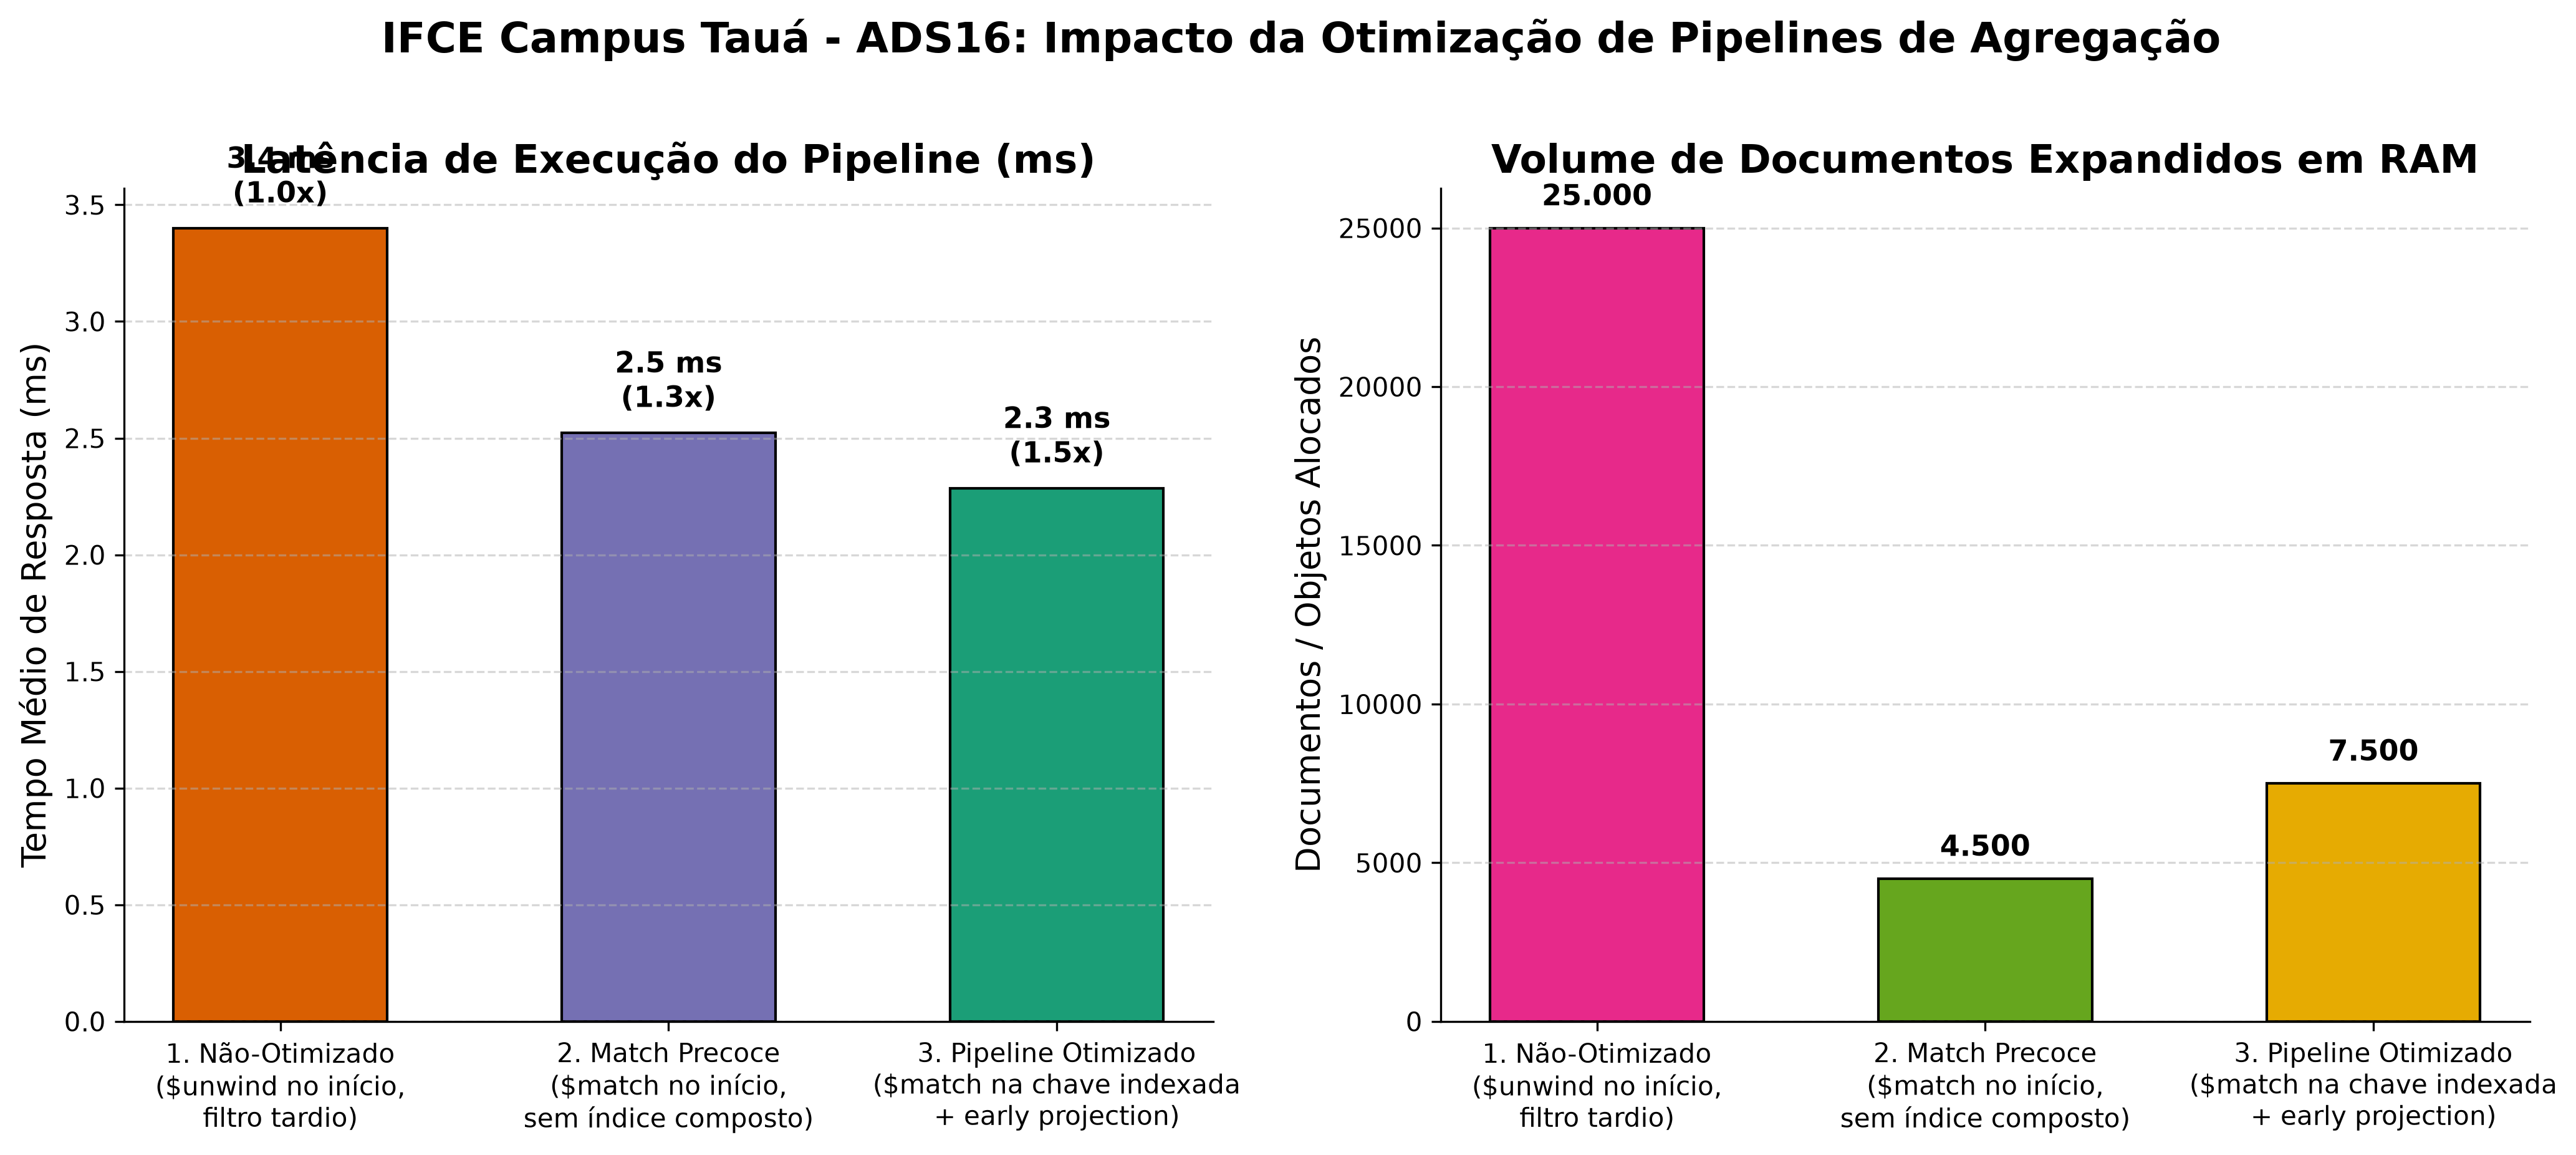
\includegraphics[width=\linewidth, height=4.2cm, keepaspectratio]{benchmark_aggregation_opt.png}
    \end{column}
  \end{columns}
\end{frame}


% ------------------------------------------------------------------------------
% Encerramento
% ------------------------------------------------------------------------------
\changecolours[inverse]{ScoutGreen}
\begin{frame}[plain]
  \vspace{2cm}
  \centering
  {\Huge \textbf{Dúvidas \& Prática em Laboratório}}\par
  \vspace{0.8cm}
  {\large IFCE Campus Tauá -- ADS16 (Modelo Orientado a Documentos)}\par
  \vspace{0.3cm}
  {\normalsize Aggregation Framework: Pipelines Analíticos, Acumuladores e Otimização}
\end{frame}

\end{document}
